\documentclass[12pt, twoside]{article}
\usepackage[letterpaper, margin=1in, headsep=0.2in]{geometry}
\setlength{\headheight}{0.6in}
%\usepackage[english]{babel}
\usepackage[utf8]{inputenc}
\usepackage{microtype}
\usepackage{amsmath}
\usepackage{amssymb}
%\usepackage{amsfonts}
\usepackage{siunitx} %units in math. eg 20\milli\meter
\usepackage{yhmath} % for arcs, overparenth command
\usepackage{tikz} %graphics
\usetikzlibrary{quotes, angles}
\usepackage{graphicx} %consider setting \graphicspath{{images/}}
\usepackage{parskip} %no paragraph indent
\usepackage{enumitem}
\usepackage{multicol}
\usepackage{venndiagram}

\usepackage{fancyhdr}
\pagestyle{fancy}
\fancyhf{}
\renewcommand{\headrulewidth}{0pt} % disable the underline of the header
\raggedbottom
\hfuzz=2mm %suppresses overfull box warnings

\usepackage{hyperref}

\fancyhead[LE]{\thepage}
\fancyhead[RO]{\thepage \\ Name: \hspace{4cm} \,\\}
\fancyhead[LO]{BECA / Dr. Huson / Geometry\\*  Unit 6: Analytic geometry\\* 10 January 2023}

\begin{document}

\subsubsection*{6.11 Classwork: Point-slope form of a linear equation \hfill HSG.GPE.B.6}
\begin{enumerate}

\subsubsection*{Point-slope form: $(y-y_1)=m(x-x_1)$}
\item Write the linear equation $y-1=2(x-3)$ in the form $y=mx+b$. 
    \begin{enumerate}[itemsep=1cm]
        \item What is the slope of the line?
        \item Name a point on the line as an ordered pair.
        \item Rewrite the equation of the line in the form $y=mx+b$. \vspace{2cm}
        \item What is the $y$-intercept of the line?
    \end{enumerate} \vspace{1cm}

\item A line has a slope of $\displaystyle \frac{3}{4}$ and passes through the point $(8, 3)$. 
    \begin{enumerate}[itemsep=1cm]
        \item Write the equation of the line in the form $(y-y_1)=m(x-x_1)$.
        \item Rewrite the equation of the line in the form $y=mx+b$. \vspace{4cm}
    \end{enumerate}

\item Find the slope of the line through the points $(1, 3)$ and $(5, 4)$.

\newpage
\item Given two points $R(7, 5)$ and $S(4, 9)$.
\begin{enumerate}
    \item Write down the distance formula. \vspace{1cm}
    \item What is the length of $\overline{RS}$?
\end{enumerate} \vspace{4cm}

\item Given two points $T(2, 3)$ and $U(10, 11)$.
\begin{enumerate}
    \item Write down the midpoint formula. \vspace{1cm}
    \item What is the midpoint of $\overline{TU}$?
\end{enumerate} \vspace{3cm}

\item A line through $P(2,2)$ is plotted on the graph below.
\begin{multicols}{2}
    \begin{enumerate}[itemsep=0.5cm]
      \item Write down the equation of the line. \vspace{0.5cm}
      \item What slope would be perpendicular to the line? \vspace{0.5cm}
      \item Write down the equation of a perpendicular line through $P$ and plot it on the graph. \vspace{1cm}
      \end{enumerate}
    \begin{flushright}
    \begin{tikzpicture}[scale=0.8]
      \draw [help lines] (-1,-1) grid (6,7);
      \draw [thick, ->] (-1.2,0) -- (6.4,0) node [below right] {$x$};
      \draw [thick, ->] (0,-1.2)--(0,7.4) node [right] {$y$};
      \draw [fill] (2,2) circle [radius=0.1] node[below right] {$P(2,2)$};
      \draw [<->, thick, domain=-0.4:5.2] plot (\x,0.5*\x+1);
    \end{tikzpicture}
    \end{flushright}
  \end{multicols} \vspace{2cm}

\newpage

\item A line has a gradient (slope) of $\displaystyle \frac{3}{4}$ and passes through the point $(8, 3)$. Find the equation of the line in the form $y=mx+b$.
\vspace{4cm}

\item A line has a gradient (slope) of $\displaystyle \frac{2}{3}$ and passes through the point $(9, 3)$. Find the equation of the line in the form $y=mx+b$.
    \vspace{4cm}

\item A line has a gradient (slope) of $\displaystyle \frac{4}{3}$ and passes through the point $(9, 13)$. Find the equation of the line in the form $y=mx+b$.
\vspace{3cm}

\item Find the equation of the line through the points $(1, 3)$ and $(5, 4)$.


\end{enumerate}
\end{document}